\documentclass[paper=a4, % Seitenformat
         fontsize=10pt,  % Schriftgröße
         oneside,        % einseitig
         headsepline,    % Trennlinie für die Kopfzeile
         notitlepage     % keine extra Titelseite
]{scrartcl}              % KOMA-Script Article
%------------------------------------------------------------------------

\usepackage[automark]{scrlayer-scrpage}  % Seiten-Stil für scrartcl
\usepackage[top=25mm]{geometry}  		% Oberer Rand 25mm Einrückung
\usepackage[utf8]{inputenc}              % Eingabekodierungen
\usepackage[T1]{fontenc}                 % Eingabekodierungen
\usepackage[english,ngerman]{babel}      % Mehrsprachenumgebung, Hauptsprache Deutsch
\usepackage{setspace}                    % Zeilenabstand
\usepackage{latexsym}                    % Latex-Symbole
\usepackage{amsfonts,amssymb,amstext}    % Mathematische Formeln
\usepackage{bbm}                         % bbm Schriftart
\usepackage{graphicx}                    % Abbildungen einbinden
\usepackage{listings}					%Programmcode einbingen
\usepackage{xcolor}						% Farben
\usepackage{changepage}
\usepackage{pdfpages}


\pagestyle{scrheadings}					% Kopfzeilen nach scr-Standard		

% Definition von Befehlen, um die Vorlage nützlicher und verständlicher zu machen
\newcommand{\codeind}[1]{\begin{adjustwidth}{3.5mm}{}#1\end{adjustwidth}}
\newcommand{\includecode}[1]{\lstinputlisting[style=codestyle, language=C]{"src/#1"}}
\newcommand{\includecodewithfilename}[1]{Datei: \texttt{#1}\vspace*{-1.5mm}\includecode{#1}}
\newcommand{\ownline}{\vspace{.7em}\hrule\vspace{.7em}} 
\newcommand{\aufgabe}[1]{\section*{Aufgabe #1}}

% Definition von Farben für die Codeblöcke
\definecolor{codegreen}{rgb}{0,0.6,0}
\definecolor{codegray}{rgb}{0.5,0.5,0.5}
\definecolor{codeblue}{rgb}{0.0, 0.0, 1.0}
\definecolor{bgcolour}{rgb}{0.97,0.97,0.97}
\definecolor{codered}{rgb}{0.7, 0.13, 0.13}

% Definition eines Designs für die Codeblöcke
\lstdefinestyle{codestyle}{
	backgroundcolor=\color{bgcolour},
	commentstyle=\color{codegreen},
	keywordstyle=\color{codeblue},
	numberstyle=\tiny\color{codegray},
	stringstyle=\color{codered},
	basicstyle=\ttfamily,
	numberstyle=\ttfamily\tiny\color{codegray},
	breakatwhitespace=false,         
	breaklines=true,                 
	captionpos=b,
	extendedchars=true                    
	keepspaces=true,                 
	numbers=left,                    
	numbersep=5pt,                  
	showspaces=false,                
	showstringspaces=false,
	showtabs=false,                  
	tabsize=4	
}

% Erlaubt es uns, in Codeblöcken Umlaute zu verwenden
\lstset{literate=%
	{Ö}{{\"O}}1
	{Ä}{{\"A}}1
	{Ü}{{\"U}}1
	{ß}{{\ss}}1
	{ü}{{\"u}}1
	{ä}{{\"a}}1
	{ö}{{\"o}}1
}


\parindent0em

\begin{document}

% Kopf des Dokuments
\textbf{Übung zur Vorlesung Informatik I} \hfill{WS 2024/25} \\  
Fakultät für Angewandte Informatik \\
Institut für Informatik \\
\textsc{Prof. Dr. J. Hähner, J. Linne, H. Cui, V. Gerling, N. Kemper} \\
\mbox{} \\
{\large Übungsgruppe 69} % Nummer der Übungsgruppe einfügen
\ownline
\begin{center}
	{\LARGE \textbf{Abgabe des 4. Übungsblatts}} \\ % Nummer des Blatts einfügen
	\mbox{} \\
	{\large Erik Wiedmann, Marwin Merkl, Manuel Henker} \\ % Namen der Teammitglieder einfügen
\end{center}
\ownline


%%%%%%%%%%%%%%%%%%%%%%%%%%%%%%%%%%%%%%%%%%%%%%%%%%%%%%%%%%%%%%%%%%%
%%%%%%%%%%%%%%%%%%% AB HIER BEARBEITEN %%%%%%%%%%%%%%%%%%%%%%%%%%%%
%%%%%%%%%%%%%%%%%%%%%%%%%%%%%%%%%%%%%%%%%%%%%%%%%%%%%%%%%%%%%%%%%%%
\aufgabe{30}\includecodewithfilename{30.h}\includecodewithfilename{30.c}

\aufgabe{32}
\begin{enumerate}
    \item[a]
    \begin{enumerate}
        \item[1.] \includecodewithfilename{32a1.c}
        \item[2.] \includecodewithfilename{32a2.c}
        \item[3.] \includecodewithfilename{32a3.c}
        \item[4.] *v + 2 = 3
        \item[5.] +(v + 2) = -1   
        \item[6.] \includecodewithfilename{32a6.c}
        \item[7.] *(p++) = 6
        \item[8.] ++(*p) = 7
        \item[9.] *(++p) = 6
        \item[10.] Mar
        \item[11.] lade
        \item[12.] ++(*p); -> (*p)++; 
        \item[13.] char w[] = v -> char w[strlen(v)]; strcpy(w, v);
        \item[14.] *p = '5' -> p = '5'
        \item[15.] *p = v -> *p = \&v             
    \end{enumerate}
    \item[b)] 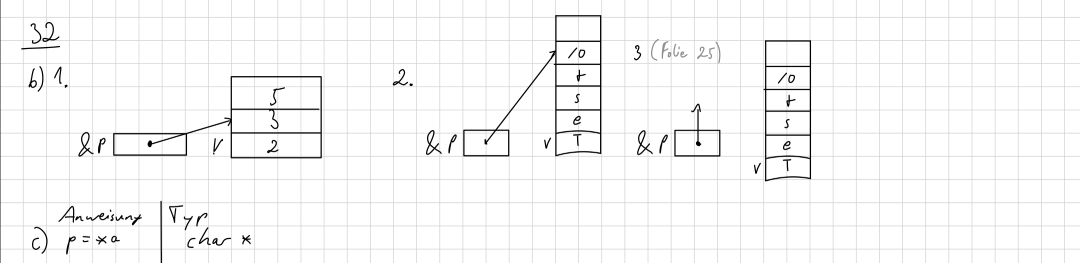
\includegraphics{32b.png}
    \item[c)] 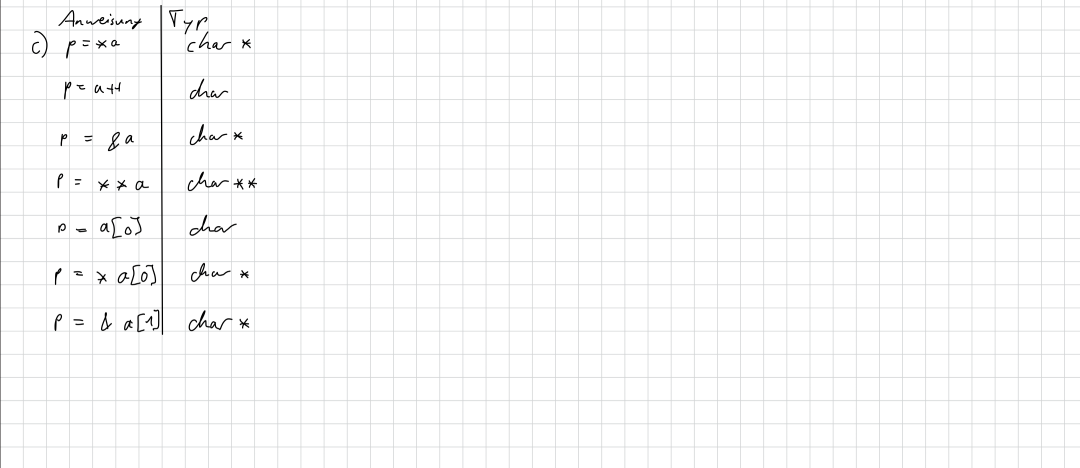
\includegraphics{32c.png} 
\end{enumerate}




%%%%%%%%%%%%%%%%%%%%%%%%%%%%%%%%%%%%%%%%%%%%%%%%%%%%%%%%%%%%%%%%%%%
%%%%%%%%%%%%%%%%%%%%%%%%%%%%%%%%%%%%%%%%%%%%%%%%%%%%%%%%%%%%%%%%%%%
%%%%%%%%%%%%%%%%%%%%%%%%%%%%%%%%%%%%%%%%%%%%%%%%%%%%%%%%%%%%%%%%%%%

\end{document}		